%\documentclass[journal,draftclsnofoot,onecolumn,11pt]{IEEEtran}
\documentclass[journal]{IEEEtran}
%\documentclass[3p,twocolumn,times,authoryear]{elsarticle}
%\documentclass[3p,twocolumn,times,authoryear]{elsarticle}
%\biboptions{}		%options for the natbib package used at Elsevier
%\bibpunct{[}{]}{,}{n}{}{;}		% to get [1,2,3]
%\bibliographystyle{elsarticle-num}

\usepackage{color}
\usepackage{graphicx}
\DeclareGraphicsExtensions{.pdf}
\graphicspath{{./Fig/}}

\usepackage[cmex10]{amsmath}
\usepackage{amssymb, latexsym}
\usepackage{amsfonts}
\usepackage{amsthm}
%\usepackage{mathrsfs}    % special font for L-operator $\mathscr{L}$
%\usepackage{subcaption}
%\usepackage{MnSymbol}
%\usepackage{bm}
%\hyphenation{op-tical net-works semi-conduc-tor}
%\usepackage{hyperref}  
%\usepackage{soul}

\newcommand{\be}{\begin{equation}}
\newcommand{\ee}{\end{equation}}
%\newcommand{\bea}{\begin{eqnarray}}
%\newcommand{\eea}{\end{eqnarray}}
\def\bal#1\eal{\begin{align}#1\end{align}}
%\newcommand{\bal}{\begin{align}}
%\newcommand{\eal}{\end{align}}
%\renewcommand{\Vec}[1]{\boldsymbol{#1}}
%\newcommand{\Mat}[1]{\boldsymbol{#1}}
\renewcommand{\Vec}[1]{\mathbf{#1}}
\newcommand{\Mat}[1]{\mathbf{#1}}
\newcommand{\Exp}[1]{\mathrm{e}^{#1}}
\newcommand{\trace}[1]{\mathop{\mathrm{tr}}\left({#1}\right)}
\renewcommand{\Re}{\mathop{\mathrm{Re}}}
\renewcommand{\Im}{\mathop{\mathrm{Im}}}
\newtheorem{theorem}{Theorem}

%\newcommand{\xabs}{|\Vec{x}|}
%\newcommand{\cfminsert}[1]{{\color{blue} {#1}}}
%\newcommand{\cfmcomment}[1]{{\color{red} {#1}}}
%\newcommand{\cfmreplace}[2]{\color{black}{{\color{black} {#2}}}\color{black}}
%% \newcommand{\cfmfinalchange}[1]{{\color{magenta}{#1}}}
%\newcommand{\cfmfinalchange}[1]{{\color{black}{#1}}}
\newcommand{\A}{\Mat{A}_{\mathcal{M}}}
\newcommand{\G}{\Mat{\Gamma}_{\mathcal{M}}}
\renewcommand{\P}{\Mat{P}}





\begin{document}
%\begin{frontmatter}
\title{Audio scene monitoring using self-calibrating microhpone arrays}
%There are wavelengths people cannot see,  sounds people cannot hear, and maybe computers have thoughts that people cannot think.

% author names and affiliations
\author{TBD} %Peter Gerstoft, Chaitanya Patil}
%\author[add2]{Santosh Nannuru}
%\author[add3]{Christoph F. Mecklenbr\"auker }
%\author[add4]{Geert Leus }
%\address[add1]{ University of California San Diego, La Jolla, CA 92093-0238,
%USA, http://noiselab.ucsd.edu}
%\address[add2]{Signal Processing and Communications Research Center, IIIT Hyderabad, India.}
%\address[add3]{ Institute of Telecommunications,
%TU Wien, 1040 Vienna, Austria, {\tt cfm@ieee.org}}
%\address[add4]{Dept. of Electrical Eng., Math. and Comp. Science, Delft Univ. of Technology, Delft, The Netherlands, g.j.t.leus@tudelft.nl}
%\thanks{Supported by the Office of Naval Research, Grant No. N00014-18-1-2118.}

\maketitle

\begin{abstract}
We present a self-calibrating system for audio source localization. The system is based on a redundant set of microphone arrays. 

We used a set of six arrays, placed at fix locations in an office. We recorded 



 \end{abstract}

\section{Introduction}
In the last several years, microphone arrays, in the form of smart speakers, have become an affordable household item. This affordability, in turn, makes it financially feasible to  place {\em several} microphone arrays in a single room.
Such a collection of arrays form an over-redundant system. This redundancy can be exploited to perform blind calibration of the arrays.

Most audio array systems assume that the geometry if the microphone is fixed and known. This assumption is reasonable when considering a single array with a fixed and known geometry. On the other hand, when a technician is installing several arrays 
in an existing room, they can be expected to follow general guidelines, such as "install the arrays far from each other" or "avoid placing microphone close to a reflective surface". They cannot be expected to provide the orientations of the arrays in space or their exact relative location.

The work presented here uses existing public beam-forming arrays. Specifically, we use ODAS~\cite{grondin2019lightweight} and matrix(?)~\cite{}. We use the existing system to identify the sound sources, compute their direction relative to the array, and produce a reconstruction of the sound for each source.

The contribution of this paper is the development of a system that takes as input the 

\subsection{Other Intro}
ML in acoustics\cite{Bianco2019}\\
An early system \cite{Ettinger2008}.\\
The steered response power  with  phase  transform  (SRP-PHAT)  \cite{brandstein1997robust}\\
video is limited in that it can only see in one direction, an acoustic array can see in all directions.\\
Source separation is an open problem.

\section{Experimental design}
We collect data continuously for 2 weeks with mini experiments. The singular vectors will be determined based on the whole period.

{\bf Information we want to extract}
\begin{itemize}
\item Locations in the room from which sound is generated.
\item recurring paths: walking while talking, while holding a smartphone generating white noise, without any additional thing
\item Speech by one or more people
\item Other sounds: Door opening / closing, keyboard / eating, utensils, cup hitting table....
\item singular vector projection for one point source at 7 localization. fig \ref{fig:projections}
\item the ~7 position should be a talking points in room or coordinate centers.
- singular vectors and histogram of ev projection based on daily life in office, based on 2 weeks of data. 
\item having a source tied to two strings, swinging back and forth
\item fan noise
\end{itemize}


\section{Theory}
The fixed array positions are assumed unknown. 

\subsection{phase only beamforming}
Each array $i$ perform SRP-HAT beamforming \cite{grondin2019lightweight} and gives up to 4 DOAs for each time instance $t$, each covering a period of 0.1 s.
Each DOA is represented with a 3D unit vector, $\|{\bf d}_t^i\|_2=1$ ,${\bf d}_t^i\in {\mathbb R}^3$, pointing towards the source and a beam time series ${\bf b}_t^i$ for the sound coming from that direction.

Frequency band ?


\subsection{PCA}
to address PCA with missing observations we Slightly following \cite{zhang2019}, more advanced methods for missing observations exist as regularized PCA \cite{lounici2013} or robust PCA\cite{xu2010}. This paper has a good review \cite{chakraborty2020}. It is not easy to compare subspaces, but it seems that we need to understand the Grassmanian \cite{chakraborty2020}.
Likely what we have below is sufficient for now.


From each array $n$ and time instance $i$, one DOA is observed  with an $x, y, z$ component. It is assumed that there are only one dominant DOA from each array, if multiple DOA exists only the most coherent with the other arrays DOA is used. This DOA is then ordered into an  observations  matrix ${\bf T}^{\rm incomplete} \in \mathbb{R}^{N_{\rm feat}\times N_{\rm obs}}$, where $N_{\rm obs}$ is number of time observations and $N_{\rm feat}$ (here 6 arrays times one 3D DOA, 18 features) number of features, $N_{\rm obs}>> N_{\rm feat}$.
Since all 6 arrays, might not have an observation at each time instance ${\bf T}^{\rm incomplete}$ will have entries that are missing, incomplete.

To construct a complete ${\bf T}^{\rm complete}$ the mean of the observed values across each row is computed ${\bf bf t}_i=\sum {\bf T}^{\rm incomplete}_{ij}/N_i$, where $N_i<N_{obs}$ is the number of observations for row $i$.
Then these mean values are filled into missing observations in ${\bf T}^{\rm complete}$, data imputation. 



Form the sample covariance matrix
\begin{equation}
{\bf R}=\frac{1}{N_{\rm obs}}{\bf T}^{\rm complete} [{\bf T}^{\rm complete}]^T
\end{equation}

The $\bf T$ matrix is decomposed into principal components
\begin{equation} 
{\bf T}^{\rm complete}={\bf U}{\bf S}{\bf V}^T
\end{equation}
\begin{equation}
{\bf R}=\sum_i{\lambda_i}{\bf u}_i{\bf u}_i^T={\bf U}{\bf S}^2{\bf U}^T
\end{equation}

\noindent
-Finding most coherent DOA for each array. using both plain cross correlation and whitened cross-correlation\\
-Finding DOAs belonging together\\
-multi path is neglected (Peter suspects, as odas will give multiple DOAs for each multi-path)

\subsection{identifying coherent arrivals on one array}
\subsection{identifying coherent arrivals on multiple arrays}

\subsection{mapping from PCA to physical domain}


\section{Experiment}

Room Fig \ref{fig:room}:
We have  six microphone arrays and since each of them gives us X,Y,Z coordinates for the source, we end up with 12 dimensions in our data matrix. Two main components are extracted by means of PCA. Upon plotting the two main components as X and Y in such a plot, we seem to be getting the XY coordinates of the sound sources. Each of these pairs is associated with a time stamp, and hence upon plotting we obtain a map of the sound sources and where they were at a any point of time.


\begin{figure} % FIGURE 1
\centering
	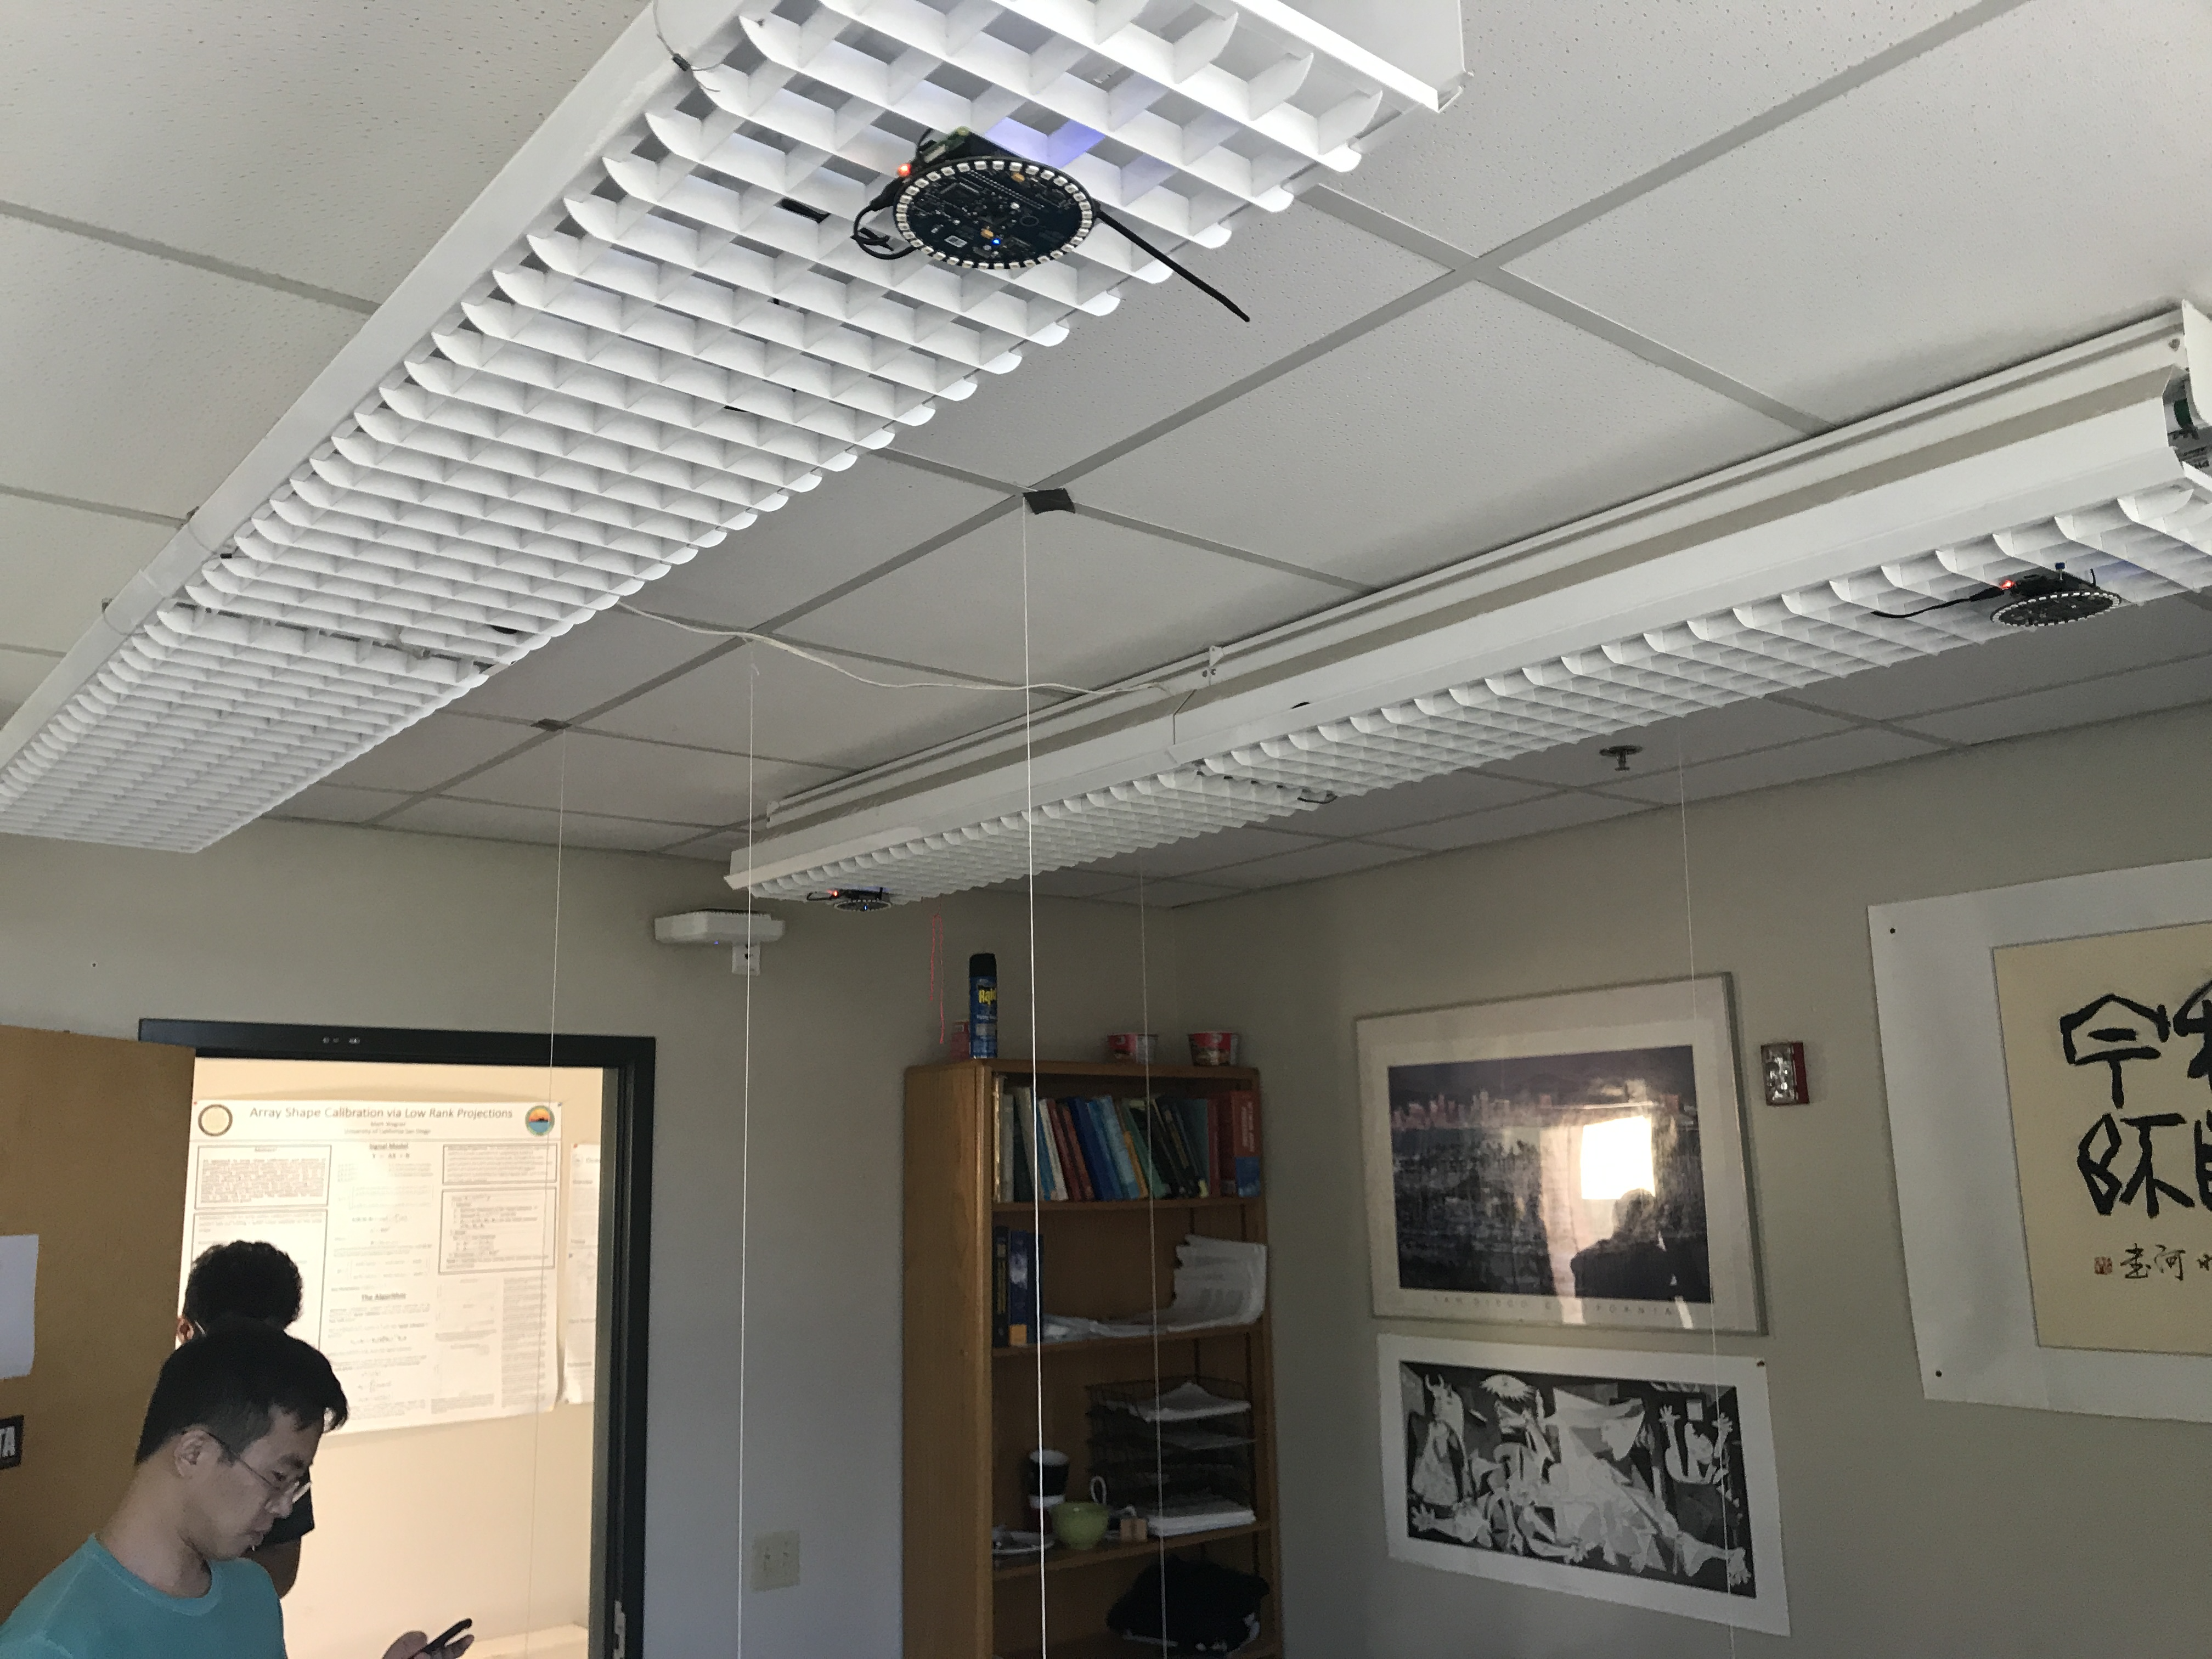
\includegraphics[width=0.6\columnwidth]{RoomPhoto.png}
	\includegraphics[width=0.6\columnwidth]{RoomCeiling.png}
	\includegraphics[width=1\columnwidth]{Fig/roomgeometry.png}
\caption{(a) Photo of room, (b) Photo of the four Odas-array mounted in ceiling (c) geometry of room. }
\label{fig:room}
\end{figure}
\begin{figure} % FIGURE 1
\centering
	\includegraphics[width=0.9\columnwidth]{projection15July.png}
\caption{Projections on the two largest eigenvectors 15 July. }
\label{fig:projections}
\end{figure}

\bibliographystyle{unsrt}
\section*{References}
\bibliography{odas,PhaseREFOct2019,biblio_rev2}


%\newpage

\clearpage




\section{APPPENDIX}
\section{Possible expansions}

\noindent
- beamforming on planar array (4 Odas in ceiling)\\
- use robust PCA\\
- sound recording quality after SVD localization \\
-\\

\section{coordinate system}
In the global coordinate system, the origin ofthe local coordinate system for  array $j$ is at ${\bf x}_j^o$ and the mapping of local coordinate vector to global is ${\bf R}_j$. Array $j$ is observing a beam with DOA ${\bf b}_j$. The source will then be on line parameterized by $s_j$
\begin{equation}
    {\bf x}_j={\bf x}_j^o+ {\bf R}_j {\bf b}_j s_j={\bf x}_j^o+  {\bf x}_j^d s_j\label{eq:line}
\end{equation}
where $ {\bf x}_j^d={\bf R}_j {\bf b}_j$ points in the beam direction in the global coordinate system. Assuming the source at location ${\bf x}$ is seen on $J $ arrays, the cost function is minimized
\begin{equation}
C= \sum_{j=1}^J \|{\bf x}-{\bf x}_j\|^2_2=\sum_{j=1}^J ({\bf x}-{\bf x}_j)^T({\bf x}-{\bf x}_j) \label{eq:cost}
\end{equation}
\begin{eqnarray}
\frac{{\rm d}  C}{{\rm d}{\bf x}}&=2\sum_{j=1}^J({\bf x}-{\bf x}_j)\\
\frac{{\rm d}  C}{{\rm d}{s_j}}   & =-2({\bf x}-{\bf x}_j)^T{\bf x}_j^d
\end{eqnarray}
Setting  the derivatives to zero and starting from initial source position $\bf x$, an iterative algorithms for minimizing the cost function\eqref{eq:cost}:
\begin{eqnarray}
s_j= ({\bf x}-{\bf x}_j^o)^T{\bf x}_j^d\\
{\bf x}=\frac{1}{J} \sum_{j=1}^J {\bf x}_j
\end{eqnarray}
In the above ${\bf x}_j$ is from \eqref{eq:line}. 
% \section{beamforming background}
% \section{Multiple-snapshot DOA estimation} % Section VI
% \label{sec:MSCS} 
% This section is copied from \cite{Gerstoft2015}.

% Even though for moving sources it befits to solve one optimization problem for each snapshot sequentially\cite{Mecklenbrauker:2013}, for stationary scenarios, the sensor data statistics can be aggregated across snapshots to provide a more stable estimate. 
% %
% Multiple snapshots are  referred to as multiple measurement vectors and the recovery might have better performance than single measurement vectors\cite{Cotter:2005}. 
% %Potentially the recovery can be made more robust by using a likelihood function Eq. \eqref{eq:Likelihood} with colored noise (full covariance matrix) or based on the Huber norm\cite{Ollila2015}.
% %
% For the  multiple-snapshot case, all snapshot are collected into one matrix, 
% %
% \begin{equation}
% \mathbf{Y} = \mathbf{A}\mathbf{X} + \mathbf{N},
% \label{eq:MultiSnapNoisyData}
% \end{equation}
% %
% where, for $L$ snapshots, $\mathbf{Y} = [\mathbf{y}(1),\cdots,\mathbf{y}(L)]$ and $\mathbf{N}= [\mathbf{n}(1),\cdots,\mathbf{n}(L)]$ are $M\times L$ matrices with the measurement and noise vectors per snapshot as columns, respectively, and $\mathbf{X}$ is the $N\times L$ signal with the complex source amplitudes at the $N$ look directions per snapshot as columns. For stationary sources the matrix $\mathbf{X}= [\mathbf{x}(1),\cdots,\mathbf{x}(L)]$ exhibits row sparsity, i.e., it has a constant sparsity profile for every column, since the few existing sources are associated with the same DOA for all snapshots.
% As the sources are stationary it makes sense to sum the source energy across all snapshots, giving the row norm ${\bf x}^{\ell_2}$
% %

% For reference, the  CBF, MVDR, and MUSIC use the data sample covariance matrix,
% %
% \begin{equation}
% \mathbf{C} = \frac{1}{L}\mathbf{Y}\mathbf{Y}^H.
% \label{eq:SCM}
% \end{equation}
% %
% The beamformer power for CBF and MVDR respectively is then,
% \begin{alignat}{2}
% P_{\rm CBF}(\theta)   &=\mathbf{w}_{\rm CBF}^H(\theta)    \mathbf{C}\mathbf{w}_{\rm CBF}(\theta) \\
% P_{\rm MVDR}(\theta)&= \mathbf{w}_{\rm MVDR}^H(\theta)\mathbf{C}\mathbf{w}_{\rm MVDR}(\theta),
% \label{eq:beam}
% \end{alignat}
% %
% where the corresponding weight vectors are given by,
% %
% \begin{alignat}{2}
%  \mathbf{w}_{\rm CBF}(\theta)&= \mathbf{a}(\theta) \\
%  \mathbf{w}_{\rm MVDR}(\theta)&= \frac{\mathbf{C}^{-1}\mathbf{a}(\theta)}{\mathbf{a}^H(\theta)\mathbf{C}^{-1}\mathbf{a}(\theta)}.
%  \label{eq:weigth}
% \end{alignat}
% %

% The CBF can also be based directly on snapshots. %as the single snapshot CBF Eq.~\eqref{eq:CBF} can be generalized to multiple snapshots,  $\mathbf{\widehat{X}}_{\text{CBF}} =\mathbf{A}^{H}\mathbf{Y}$.
% The power estimates $P_{\rm CBF}(\theta_i)$, $P_{\rm MVDR}(\theta_i)$, and the corresponding $i$th squared component of $\mathbf{x}^{\ell_{2}}_{\text{CS}} $ are thus comparable. Note that since the MVDR weights in Eq.~\eqref{eq:weigth} involve the inverse of the sample covariance matrix, MVDR requires a full rank $\mathbf C$, i.e., $L\geq M$ snapshots.

% \section{ODAS}

% \subsection{Description of ODAS array}
% Number of arrays: 6
% Number of microphones in array: 8
% Shape of the array: circular diameter 10 cm.

% \subsection{Algorithm used in ODAS}

% The developers of ODAS \cite{grondin2019lightweight} came up with a modified version of SRP-PHAT, known as SRP-PHAT-HSDA. 

% Below is a summary of \cite{grondin2019lightweight}. {\it The paper is not that easy to read.}


% \subsubsection{SRP-PHAT}

% Say there are M microphones on the array. Each of them receives a sound signal $x_{m}$. Each incoming signal at each microphone is divided into frames of N samples. The frames are offset from each other by $\Delta N$ samples. Each frame is also multiplied by the sine window. The operation can be expressed as:
% \begin{equation} \label{eq:1}
% x^{l}_{m}[n] = w[n]x_{m}[n + l\Delta N]
% \end{equation}
% where $l$ represents the frame index, m represents the microphone index.

% Then, we compute the STFT using the FFT algorithm. Once we have done so, we can use the IFFT algorithm to compute the GCC-PHAT. The GCC PHAT is computed for pairs of microphones. If the time delay is n, we compute the GCC-PHAT between two microphones $p$ and $q$ as the following:
% \begin{equation} \label{eq:2}
% r^{l}_{pq} = \frac{1}{N} \sum_{k=0}^{N-1} \frac{X^{l}_{p}[k]X^{l}_{p}[k]^{*}}{|X^{l}_{p}[k]X^{l}_{p}[k]|+\epsilon} e^{\frac{2\pi jkn}{N}} 
% \end{equation}
% Explanation: element-wise multiplication of the normalized DFT coefficients from the first microphone with that of the second microphone and finally with a complex exponential signal whose frequency is specified by the delay between the two microphones n.

% What sort of an output does GCC PHAT have? Just a guess:
% The IDFT is a linear combination of Fourier basis vectors and gives an n dimensional signal. In this 'signal' each bin corresponds to a time delay. We have such a signal corresponding to each pair of microphones. If we have $n$ microphones, we have $n$ choose $2$ GCC-PHAT outputs. 

% For each frame, l, SRP-PHAT searches for potential sources over a certain 'discrete space' (limited number of things to search over?). SRP-PHAT uses GCC-PHAT (Generalized Cross Correlation Phase Transform). 

% \subsection{Modifications in SRP PHAT HSDA}

% A few modifications are introduced in SRP PHAT HSDA in order to reduce the number of computations. There are changes in:
% \begin{itemize}
%     \item Directivity
%     \item Maximum Sliding Window Automatic Calibration
%     \item Hierarchical Search
% \end{itemize}

% \subsubsection{Directivity}


% output of ODAS

% Our experiment: We have a total of four microphone arrays and since each of them gives us X,Y,Z coordinates for the source, we end up with 12 dimensions in our data matrix. Two main components are extracted by means of PCA. Upon plotting the two main components as X and Y in such a plot, we seem to be getting the XY coordinates of the sound sources. Each of these pairs is associated with a time stamp, and hence upon plotting we obtain a map of the sound sources and where they were at a any point of time.

% \subsection{ Multiple ODAS}

% Correcting for time delay.

% \subsection{cross-correlation}
% \subsubsection{Beam time delay}
% \subsubsection{amplitude}

\section{Modelling and Simulation}
Room Impulse Response (RIR) Generator
%\web
{https://www.audiolabs-erlangen.de/fau/professor/habets/software/rir-generator}

RIR generator can model a room as a Linear Time-Invariant (LTI) system. If we provide the reverberation time (RT), room dimensions, the position of microphones and sound sources, RIR generator can characterize the room as a impulse response $h(t)$ of a certain LTI system. Then, if we have a sound signal $x(t)$, the system output $y(t)$ is $y(t) = x(t) * h(t)$. 

The most common such property to be inferred is the RT, which is the time taken for reverberant energy to decay some amount.  RT can be estimated from histograms of decay rates measured from short windows of the signal.\cite{ratnam2003blind}

Python package “Pyroomacoustics: A python package for audio room simulation and array processing algorithms,\cite{Scheibler2018}

\subsection{Localization of the Sound Sources}
Suppose we consider a 2-D and single source problem, i.e., the positions of both the microphones and sources have the identical coordinate in one dimension and there is only one sound source in the room. We assume they share the same $x$. Denote  $(x, y_0, z_0)$ as the  of the source position and $(x, y_i, z_i)$ as the position of the microphones $(i = 1, \ldots , n)$ for $n$  microphones. By assigning the appropriate RT, we  obtain the true room impulse responses $h_0^i(t)$ for each microphone. 

Assume that we have such a candidate source points  $(x, \bar{y_j}, \bar{z_j}) (j = 1, \ldots K)$. Suppose we  search $N$ points in the $y$ coordinate and $M$ points in the $z$ coordinate and then we have $K = NM$. For each of the candidate point, combining with microphones positions $(x, y_i, z_i)$ and the given RT, it can generate a impulse response $h_j^i(t)$. Consider a source input $x(t)$, by applying different impulse responses $h_j^i(t)$, we obtain system outputs $y_j^i(t)$. For each candidate point, we calculate pair-wise time delay between $y_j^l(t)$ and $y_j^m(t)$ $(l,m = 1,\ldots n, l < m)$ and obtain the $n(n-1)/2$ dimension time delay vector $\tau_{j} = [\tau_j^{12}, \ldots, \tau_j^{(n-1)n}]$. 

Similarly, for the true impulse response $h_0^i(t)$, we have the true system output $y_0^i(t)$ and the true time delay vector $\tau_0 = [\tau_0^{12}, \ldots \tau_0^{(n-1)n}]$.

The estimated sound source is selected from these candidate points with the following criteria: 
\begin{equation}
    \min_j \|\tau_j - \tau_0\|_2^2
\end{equation}
where $\| \|_2$ is the $l_2$ norm. As long as we identify the index of the candidate point, the position of the sound source can be estimated as  $(x, \bar{y_j}, \bar{z_j})$. 


%%%%%%%%%%%%%%%%%
\section{Processing localization}
We collect all observations in a matrix ${\bf T} \in \mathbb{R}^{N_{\rm feat}\times N_{\rm obs}}$, where $N_{\rm obs}$ is number of observations and $N_{\rm feat}$ number of features selected for optimization, $N_{\rm obs} >> N_{\rm feat}$

The fixed array positions are assumed unknown. 

Blind localization.


\subsection{K-means}
% \subsection{PCA-SVD}
% Form the sample covariance matrix
% \begin{equation}
% {\bf R}=\frac{1}{N_{\rm obs}}{\bf T} {\bf T}^H
% \end{equation}
% \begin{equation} 
% {\bf T}={\bf U}{\bf S}{\bf V}^H
% \end{equation}
% \begin{equation}
% {\bf R}=\sum_i{\lambda_i}{\bf u}_i{\bf u}_i^H={\bf U}{\bf S}^2{\bf U}^H
% \end{equation}
% \subsection{Remove NaN}
% Why NaN
% \subsection{Ojas method}
% \cite{oja1982simplified}
% Can this be used? \cite{Balsubramani2013}

% \begin{equation} \label{eq:}
% V_n = \frac{V_{n-1} + \gamma_n X_n X^T_n V{n-1}}{||V_{n-1} + \gamma_n X_n X^T_n V{n-1}||}
% \end{equation}

% We used Oja's rule as a way of calculating eigenvectors in an online manner. We traverse through close to 2.6 million data points and at each step update the eigenvector using the equation above.

% This way we get the eigenvector corresponding to the largest eigenvalue. Then, for each data point, we calculate the projection vector onto this eigenvector and subtract it from the original data points. This way we are left with data orthogonal to the first eigenvector. We use Oja's rule again on this modified dataset and obtain the second largest eigenvector.

% We noticed our resultant eigenvectors to be non-orthogonal. The dot product of our eigenvectors was found to be about 0.212 or -0.212. This was probably due to the presence of NaNs in the dataset. The approach has since been abandoned. 

\subsection{robust PCA}



\subsection{Supervised learning}
\subsection{Unsupervised learning}
\subsection{Semi-supervised learning}
\section{Time series reconstruction}
\subsection{combining beams}

%%%%%%%%%%%%%
%All noise covariance matrices are collected in the 3-way array
%\begin{align}
%{\Mat{\Sigma}}_{\Mat N} = [  \Mat\Sigma_{\Vec{n}_l}| \,l=1,\ldots,L ]
%\in \mathbb{C}^{N\times N\times L}.
%\label{eq:sigma_N}
%\end{align}

% \subsection{Example}
% $N_{\rm obs}=2.6\cdot 10^6$ 

% $N_{feat}=12$, 4 beams of 3 coordinates.

% 8 ms between samples
 
% 2 month of observation
 
% Mostly unobserved.
% how to do it online gives a 

% Change point detection.
% \begin{figure} % FIGURE 1
% \centering
% 	\includegraphics[width=1\columnwidth]{DriftGrondin.png}
% \caption{50 sample drift delay 16000 samples/ Hz. x-axis is 0.5*550=250s}
% \label{fig:drift}
% \end{figure}



%\section*{Acknowledgment}

\section{Interpolating locations}

Each point in either space is $2 \times 1$ column vector.

We have two triangles, each described by a $2\times 3$ matrix $R$ (for room) and 
$L$ for localization or PCA.



We are looking for a linear transformation from localization coordinates to room coordinates.

$T: \vec{l} \to \vec{r}$

$T = \vec{s}+ B\vec{l}$ Where $B$ is a $2 \times 2$ matrix and $\vec{s}$ is a  $2 \times 1$ vector.

Constraints: for $i=1,2,3$ : $T(\vec{l}_i) = \vec{r}_i$
Which is equivalent to $\vec{s}+B \vec{l}_i = \vec{r}_i$.

Packaging all 3 equations together we get:
$$\vec{s} + B L = R$$, We know $L$ and $R$, we need to solve for $\vec{s}$ and $B$.

\section{Linear mapping}
In general the mapping between $N$ 3-D room observations $\bf r$ and 18-D beam domain $\bf l $ is non-linear and unknown ${\bf R}= f({\bf L}$. For locations close together a linear mapping might be sufficient. 
\begin{equation}
    {\bf r}= {\bf a}+ {\bf B}{\bf l}
\end{equation}
where ${\bf a}$ is the offset and ${\bf B}$ is the linear coefficients.

Focusing on a $N$ observation locations near a speaker ${\bf R}=[{\bf r}_1,\ldots, {\bf r}_N]\in {\cal R}^{3\times N}$
and just the 3 first components in PCA ${\bf L}=[{\bf l}_1,\ldots, {\bf l}_N]\in {\cal R}^{3\times N}$
\begin{equation}
    {\bf R}= {\bf a}+ {\bf B}{\bf L}
\end{equation}
${\bf a}{\cal R}^{3}$ and ${\bf B}{\cal R}^{3\times 3}$, thus 12 unknowns. For on 2D domain there are 6 unknowns.
\end{document}

